\documentclass[10pt,aspectratio=169]{beamer}

\usetheme{Madrid}
\usecolortheme{seahorse}
\useinnertheme{circles}
\setbeamertemplate{navigation symbols}{}
\setbeamertemplate{footline}[frame number]

\usepackage{amsmath,amssymb}
\usepackage{bm}
\usepackage{tikz}
\usetikzlibrary{arrows.meta, positioning}

\newcommand{\ket}[1]{\left|#1\right\rangle}
\newcommand{\bra}[1]{\left\langle#1\right|}

\title[QSVT Poisson Demo]{A Toy Demonstration of Quantum Singular Value Transformation on the 1D Poisson Equation}
\author{Yang Mo}
\date{}

\begin{document}

% ---------------------------------------------------------------- 1
\begin{frame}
  \titlepage
  \begin{center}
    \small Demonstrating the QSVT mechanism on a tiny finite-difference system
  \end{center}
\end{frame}

% ---------------------------------------------------------------- 2  (roadmap)
\begin{frame}{The General Recipe}
  Solving a PDE numerically almost always follows the same path:

  \vspace{0.8em}
  \begin{center}
  \begin{tikzpicture}[
    node distance=1.3cm and 1.9cm,
    box/.style={draw, thick, rounded corners, align=center,
                minimum height=1.05cm, minimum width=2.5cm, fill=structure!12},
    qbox/.style={draw, very thick, rounded corners, align=center,
                 minimum height=1.05cm, minimum width=2.5cm, fill=structure!35},
    arr/.style={-{Latex[length=2.6mm]}, thick}
  ]
    \node[box]              (pde) {Continuous PDE\\[2pt]$-u''=f$};
    \node[box, right=of pde](lin) {Linear system\\[2pt]$A\bm{u}=\bm{f}$};
    \node[qbox,right=of lin](sol) {Solution\\[2pt]$\bm{u}=A^{-1}\bm{f}$};
    \draw[arr] (pde) -- node[above]{\small discretize}
                          node[below]{\small\emph{finite diff.}} (lin);
    \draw[arr, draw=red!70] (lin) -- node[above]{\small solve}
                          node[below, red!70!black]{\small\textbf{quantum}} (sol);
  \end{tikzpicture}
  \end{center}

  \vspace{0.4em}
  \pause
  \begin{itemize}
    \item \textbf{Steps 1--2 (classical):} mesh the domain and replace derivatives
          by finite differences $\Rightarrow$ a matrix equation $A\bm{u}=\bm{f}$.
    \item \textbf{Step 3 (quantum):} the matrix equation is where QSVT enters ---
          block-encode $A$ and apply a polynomial inverse to get $A^{-1}\bm{f}$.
  \end{itemize}

  \centering
  \emph{This talk: a two-point Poisson example carried through every step.}
\end{frame}

% ---------------------------------------------------------------- 3
\begin{frame}{The Problem: 1D Poisson Equation}
  We solve the boundary-value problem
  \[
    -u''(x) = f(x), \qquad x \in (0,1), \qquad u(0)=u(1)=0.
  \]

  \pause
  \textbf{Second-order finite differences} on interior grid points ($h$ = spacing):
  \[
    -\,\frac{u_{j-1} - 2u_j + u_{j+1}}{h^2} = f_j
    \quad\Longrightarrow\quad A\,\bm{u} = \bm{f}.
  \]

  \pause
  With two interior points the tridiagonal Laplacian collapses to a $2\times 2$ system:
  \[
    A =
    \begin{pmatrix} 2 & -1 \\ -1 & 2 \end{pmatrix},
    \qquad
    \bm{f} = \begin{pmatrix} 1 \\ 0.3 \end{pmatrix}.
  \]

  \centering
  \emph{Goal:} produce the normalized state $\ket{u} \propto A^{-1}\ket{f}$ with a quantum circuit.
\end{frame}

% ---------------------------------------------------------------- 4  (theory)
\begin{frame}{The QSVT Idea --- Why $W(A)$, Why a Polynomial}
  A quantum circuit is \emph{unitary}, but $A$ is not. Two ideas bridge the gap.

  \textbf{1. Block-encoding.} Rescale $A$ to $\|A\|\le 1$ and hide it as the top-left block of a
  unitary --- the \emph{signal unitary}:
  \[
    W(A)=\begin{pmatrix} A & i\sqrt{I-A^2}\\[2pt] i\sqrt{I-A^2} & A\end{pmatrix},
    \qquad (\bra{0}\!\otimes\! I)\,W(A)\,(\ket{0}\!\otimes\! I)=A.
  \]

  \pause
  \textbf{2. QSVT.} Interleaving $W$ with ancilla phase rotations $S(\phi)=e^{i\phi Z}$ applies a
  \emph{polynomial to the eigenvalues} of $A$:
  \[
    U_\Phi=S(\phi_0)\,W\,S(\phi_1)\,W\cdots W\,S(\phi_d),
    \quad
    [U_\Phi]_{\text{top-left}}=P(A)=\sum_j P(\lambda_j)\ket{\lambda_j}\!\bra{\lambda_j}.
  \]

  \pause
  \textbf{Inversion.} QSVT sends each eigenvalue $\lambda_j \to P(\lambda_j)$. Since $A^{-1}$ inverts
  every eigenvalue, choosing $P(x)\approx \gamma/x$ on the spectrum builds $P(A)\approx \gamma\,A^{-1}$.
  So $P(A)\ket{f}\propto A^{-1}\ket{f}$ --- the solution --- kept by postselecting the ancilla on $\ket{0}$.
\end{frame}

% ---------------------------------------------------------------- 5  (implementation)
\begin{frame}{Implementation for the Two-Point Poisson}
  On the eigenvalues $\{\tfrac14,\tfrac34\}$ of $B=A/4$, approximate $\gamma/x$ ($\gamma=\tfrac{3}{32}$)
  by the exact degree-3 polynomial
  \[
    p(x) = \tfrac53\,x - \tfrac83\,x^3 .
  \]

  The four phases realizing $p$, and their sequence:
  \[
    \Phi=[0.0082,\,-0.6155,\,0.6155,\,3.1334], \qquad
    U_\Phi=S(\phi_0)W(B)S(\phi_1)W(B)S(\phi_2)W(B)S(\phi_3).
  \]

  \pause
  Realized as a circuit ($S(\phi)\to R_z(-2\phi)$, system $q_1$ prepared as $\ket{f}$):
  \begin{center}
    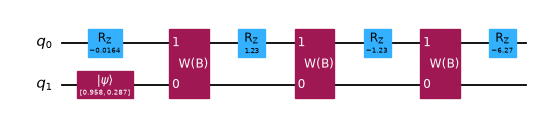
\includegraphics[width=0.82\textwidth]{circuit}
  \end{center}
\end{frame}

% ---------------------------------------------------------------- 7  (the ONE result slide)
\begin{frame}{Result}
  \textbf{Classical reference.} Solve $A\bm{u}=\bm{f}$ with ordinary numerical linear
  algebra (\texttt{numpy}), then normalize --- the quantum output carries no overall scale:
  \[
    \bm{u}/\|\bm{u}\| = (0.8209,\ 0.5711).
  \]

  \textbf{Quantum output.} Postselect the ancilla on $\ket{0}$ and normalize the two
  circuit amplitudes:
  \[
    (0.8209,\ 0.5711).
  \]

  \vspace{0.3em}
  The two normalized vectors agree componentwise to $\sim 10^{-9}$, set by the rounded
  phase angles. Postselection succeeds with probability $\approx 0.11$.
\end{frame}

% ---------------------------------------------------------------- 8
\begin{frame}{Summary \& Outlook}
  \textbf{Done:} block-encode $A$, apply an exact inverse polynomial via a degree-3
  QSVT phase sequence, run as a Qiskit circuit --- its output matches the classical
  solution to $\sim 10^{-9}$.

  \vspace{0.6em}
  \textbf{Hard at scale:} state preparation of $\ket{f}$, phase-angle synthesis for
  general polynomials, and higher degrees as the spectrum widens.

  \vspace{0.8em}
  {\small \emph{Refs:} Lin, arXiv:2201.08309 (\S8.4);\;
   Childs--Liu--Ostrander, arXiv:2002.07868;\;
   Shaviner--Chen--Frankel, arXiv:2507.09686.}

  \begin{center}\Large Thank you!\end{center}
\end{frame}

\end{document}
